\documentclass[12pt]{article}
\usepackage[utf8]{inputenc}
\usepackage[spanish]{babel}
\usepackage[a4paper]{geometry}
%\geometry{top=1.5cm, bottom=1.0cm, left=1.25cm, right=1.25cm}
\usepackage{pdflscape}
\usepackage{xcolor}
\usepackage{tikz}
\usetikzlibrary{positioning, shapes.multipart}
\usepackage{csvsimple}
\usepackage{pgfplotstable,booktabs}
\pgfplotsset{compat=1.16}

\begin{document}
\title{Ejercicios de PERT}
\author{Ana Maritza Bello Yañez}
\maketitle
%\setlength{\parindent}{0pt}
%\setlength{\parskip}{1em}


\section{Ejercicio 1}
La empresa SALMA está preparando la planificación, aplicando la técnica PERT, de
un proyecto informático, cuyas actividades se indican en la tabla inferior, así
como sus precedentes y la duración expresada en semanas (optimista, pesimista y
más probable):  \\
\\


\begin{center}
\begin{tabular}{cccccccc}

Actividad & Precedentes & $T_o$ & $T_n$ & $T_p$ & $T_\mu$ & $\sigma^2$ & $\sigma$ \\
\hline
\hline
A &  -  & 1 & 2 & 3 & 2 & 0.33 & 0.58 \\
B &  A  & 2 & 4 & 6 & 4 & 0.67 & 0.82 \\
C & B,H & 1 & 1 & 1 & 1 & 0.00 & 0.00 \\
D &  -  & 3 & 6 & 9 & 6 & 1.00 & 1.00 \\
E &  G  & 2 & 3 & 4 & 3 & 0.33 & 0.58 \\
F &  E  & 3 & 5 & 7 & 5 & 0.67 & 0.82 \\
G &  D  & 1 & 2 & 3 & 2 & 0.33 & 0.58 \\
H &  G  & 1 & 2 & 3 & 2 & 0.33 & 0.58 \\
I &  D  & 1 & 3 & 5 & 3 & 0.67 & 0.82 \\
J &  I  & 3 & 4 & 5 & 4 & 0.33 & 0.58 \\
K &  D  & 2 & 3 & 4 & 3 & 0.33 & 0.58 \\
L & J,K & 3 & 5 & 7 & 5 & 0.67 & 0.82 \\
M & C,L & 1 & 2 & 3 & 2 & 0.33 & 0.58 \\
\hline

\end{tabular}
\end{center}

\begin{itemize}
    \item Diseño completo del grafo, incluyendo holguras y camino crítico.
    
    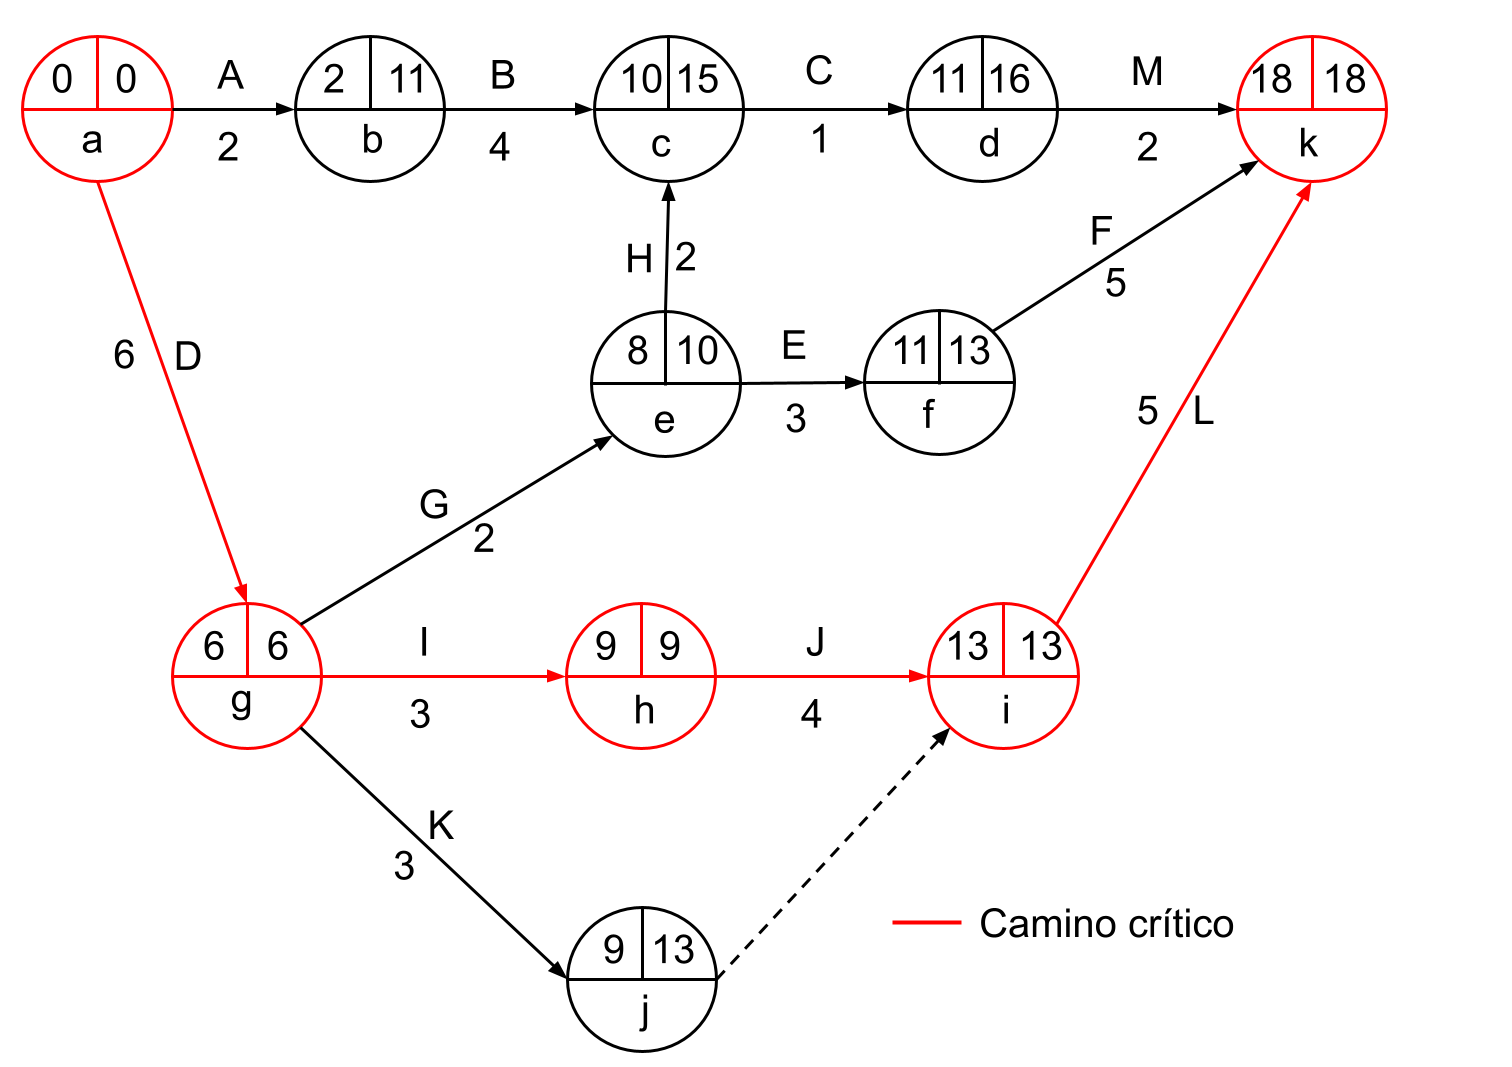
\includegraphics[scale=0.3]{../figures/pert_01.png}

    \item Matriz asociada al grafo
    
    \begin{center}
    \begin{tabular}{ccccccccccccccc}
          & A & B & C & D & E & F & G & H & I & J & K & L & M \\
      \hline
        A   & 0 & 0 & 0 & 0 & 0 & 0 & 0 & 0 & 0 & 0 & 0 & 0 & 0 \\
        B   & \textcolor{red}{1} & 0 & 0 & 0 & 0 & 0 & 0 & 0 & 0 & 0 & 0 & 0 & 0 \\
        C   & 0 & \textcolor{red}{1} & 0 & 0 & 0 & 0 & 0 & \textcolor{red}{1}& 0 & 0 & 0 & 0 & 0 \\
        D   & 0 & 0 & 0 & 0& 0& 0& 0& 0& 0& 0& 0& 0& 0 \\
        E   & 0 & 0 & 0 & 0& 0& 0& \textcolor{red}{1}& 0& 0& 0& 0& 0& 0 \\
        F   & 0 & 0 & 0 & 0& \textcolor{red}{1}& 0& 0& 0& 0& 0& 0& 0& 0 \\
        G   & 0 & 0 & 0 & \textcolor{red}{1}& 0& 0& 0& 0& 0& 0& 0& 0& 0 \\
        H   & 0 & 0 & 0 & 0& 0& 0& \textcolor{red}{1}& 0& 0& 0& 0& 0& 0 \\
        I   & 0 & 0 & 0 & \textcolor{red}{1}& 0& 0& 0& 0& 0& 0& 0& 0& 0 \\
        J   & 0 & 0 & 0 & 0& 0& 0& 0& 0& \textcolor{red}{1}& 0& 0& 0& 0 \\
        K   & 0 & 0 & 0 & \textcolor{red}{1}& 0& 0& 0& 0& 0& 0& 0& 0& 0 \\
        L   & 0 & 0 & 0 & 0& 0& 0& 0& 0& 0& \textcolor{red}{1}& \textcolor{red}{1}& 0& 0 \\
        M   & 0 & 0 & \textcolor{red}{1} & 0& 0& 0& 0& 0& 0& 0& 0& \textcolor{red}{1}& 0 \\
    \end{tabular}
  \end{center}

    \item ¿Qué efectos tendrán sobre el proyecto los siguientes eventos:

    - La actividad A se retrasa 9 semanas

No afectaría al proyecto puesto que para terminar la actividad A, tenemos
justamente 9 semanas de holgura.

    - La actividad D se retrasa 3 semanas

Dado que la actividad se encuentra en el camino crítico, retrasaría todo el
proyecto 3 semanas.

    - La actividad L se reduce en 1 semana

Esta actividad también se encuentra en el camino crítico y no tiene holgura, por
lo que su retraso tendría como consecuencia el retraso de todo el proyecto.

\end{itemize}

\pagebreak
\section{Ejercicio 2}

La empresa CLARK S.A. de C.V. debe reubicar sus oficinas hacia nuevas
instalaciones en la zona norte con el objetivo de brindar una atención
especializada a sus clientes, el director debe preparar un informe detallado de
las labores y el tiempo de cada uno para el traslado, incluyendo rutas críticas
y estimaciones de tiempos. El director ha desarrollado el proyecto con 11
actividades que se presentan en el siguiente cuadro: \\
\\
\begin{center}
  \begin{tabular}{ccccccccc}
      Actividad & Detalle & Precedentes & $T_o$ & $T_n$ & $T_p$ & $T_\mu$ & $\sigma^2$ & $\sigma$ \\
\hline
\hline
A &  Seleccionar tipo de oficinas  &  -     & 1 & 3 & 5 & 3 & 0.67 & 0.82 \\
B &  Crear plan organizacional     &  -     & 3 & 4.5 & 9 & 5 & 1.00 & 1.00 \\
C &  Determinar personal           &  B     & 2 & 3 & 4 & 3 & 0.33 & 0.58 \\
D &  Diseñar las instalaciones     &  A,C   & 2 & 4 & 6 & 4 & 0.67 & 0.82 \\
E &  Contruir los interiores       &  D     & 4 & 7 & 16 & 8 & 2.00 & 1.41 \\
F &  Seleccionar personal          &  C     & 1 & 1.5 & 5 & 2 & 0.67 & 0.82 \\
G &  Contratar nuevos empleados    &  F     & 2.5 & 3.5 & 7.5 & 4 & 0.83 & 0.91 \\
H &  Traslado de archivos y material  &  F     & 1 & 2 & 3 & 2 & 0.33 & 0.58 \\
I &  Hacer arreglos financieros    &  B     & 4 & 5 & 6 & 5 & 0.33 & 0.58 \\
J &  Capacita nuevo personal       &  H,E,G & 1.5 & 3 & 4.5 & 3 & 0.50 & 0.71 \\
\hline

  \end{tabular}
\end{center}

\begin{itemize}
    \item Diseño completo del grafo, incluyendo holguras y camino crítico.

    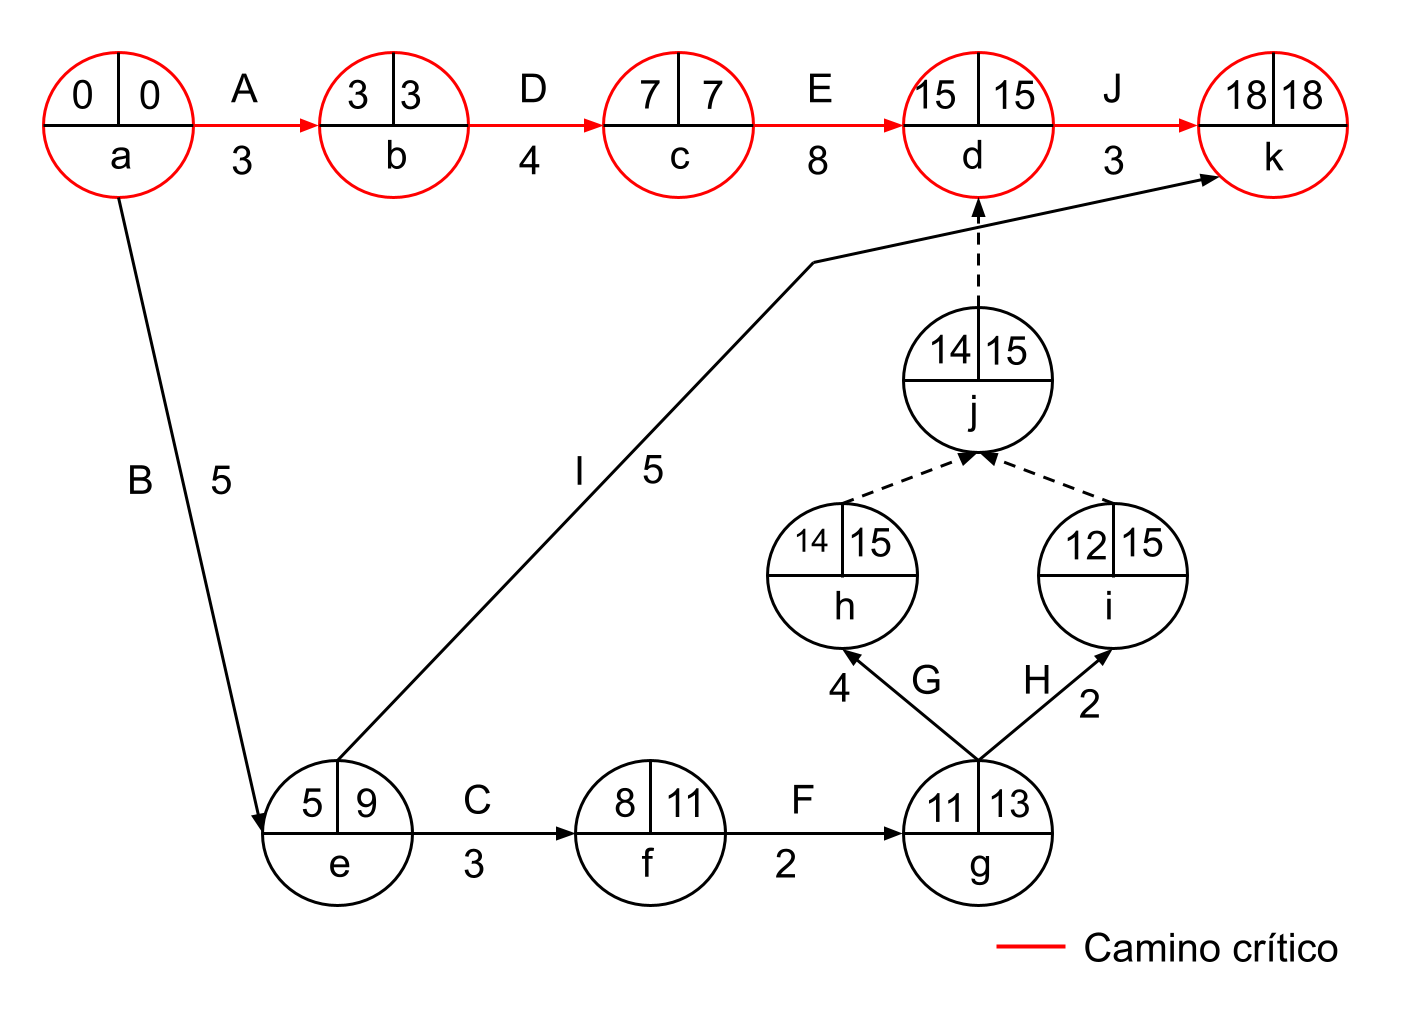
\includegraphics[scale=0.3]{../figures/pert_02.png}

    \item Matriz de encaminamientos asociada al grafo

    \begin{center}
      \begin{tabular}{c|cccccccccc}
             & A & B & C & D & E & F & G & H & I & J \\
        \hline
          A  & 0& 0& 0& 0& 0& 0& 0& 0& 0 & 0 \\
          B  & 0& 0& 0& 0& 0& 0& 0& 0& 0 & 0 \\ 
          C  & 0& \textcolor{red}{1}& 0& 0& 0& 0& 0& 0& 0 & 0 \\ 
          D  & \textcolor{red}{1}& 0& \textcolor{red}{1}& 0& 0& 0& 0& 0& 0 & 0 \\ 
          E  & 0& 0& 0& \textcolor{red}{1}& 0& 0& 0& 0& 0 & 0 \\
          F  & 0& 0& \textcolor{red}{1}& 0& 0& 0& 0& 0& 0 & 0 \\
          G  & 0& 0& 0& 0& 0& \textcolor{red}{1}& 0& 0& 0 & 0 \\
          H  & 0& 0& 0& 0& 0& \textcolor{red}{1}& 0& 0& 0 & 0 \\
          I  & 0& \textcolor{red}{1}& 0& 0& 0& 0& 0& 0& 0 & 0 \\
          J  & 0& 0& 0& 0& \textcolor{red}{1}& 0& \textcolor{red}{1}& \textcolor{red}{1}& 0 & 0 
      \end{tabular}
    \end{center}

    \item \textbf{Duración estimada del proyecto en días}

    18 días

    \item Responder las siguientes preguntas relacionadas con el proyecto:

    - \textbf{¿Cuál será la probabilidad de terminar el proyecto hasta 18 días?}

      La probabilidad es del 50\%
      (ver la siguiente tabla)

    - \textbf{¿Cuál será la probabildad de terminar el proyecto hasta 25 días?}
      
      La probabilidad es del 100\%
      (ver la siguiente tabla)

- \textbf{¿Cuál será la duración del proyecto para una probabilidad de finalización del
95\%?}

Sería de 21 días (ver la siguiente tabla)

\begin{center}
  \begin{tabular}{ccccccc}
    $T_{RC}$  & $\sigma^2_{RC}$ & $\sigma_{RC}$ & Dias solicitados & Z    & Normal
dist & Norm dist inv \\
\hline
\hline
18 & 3.83 & 1.95            & 18            & 0                & 0.50 &                          \\
18 & 3.67 & 1.91            & 25            & -3.65            & 1.00 &                          \\
   &      &                 &               &                  & 0.95 & 21.22                    \\
\hline

  \end{tabular}
\end{center}
    
\end{itemize}

\end{document}
    